\normaltrue
\correctionfalse

%\UPSTIidClasse{11} % 11 sup, 12 spé
%\newcommand{\UPSTIidClasse}{12}

\exer{Mouvement RT  $\star$ \label{B2:13:PTSI:05:02}}
\setcounter{numques}{0}
\UPSTIcompetence{B2-13}
\index{Compétence B2-13-PTSI}
\index{Mécanisme à 1 rotation et 1 translation}
\ifcorrection
\else
\textbf{Pas de corrigé pour cet exercice.}
\fi

\ifprof
\else
Soit le mécanisme suivant. On a $\vect{AB}=\lambda(t)\vect{i_1}$.
\begin{center}
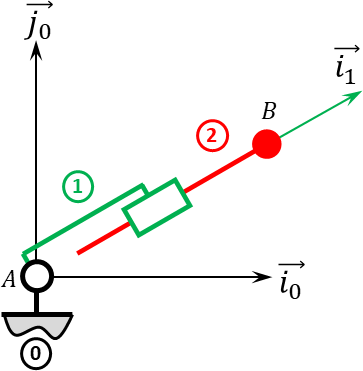
\includegraphics[width=6cm]{05_RT_01}
\end{center}
\fi

\question{Réaliser le paramétrage du mécanisme.}
\ifprof  ~\\

\else
\fi



\ifprof
\else
\footnotesize

\normalsize

\begin{flushright}
\footnotesize{Corrigé  voir \ref{B2:13:PTSI:05:02}.}
\end{flushright}%
\fi